\documentclass{beamer}
\usetheme[pageofpages=of,% String used between the current page and the
                         % total page count.
          bullet=circle,% Use circles instead of squares for bullets.
          titleline=true,% Show a line below the frame title.
          alternativetitlepage=true,% Use the fancy title page.
       %   titlepagelogo=logo-polito,% Logo for the first page.
       %   watermark=watermark-polito,% Watermark used in every page.
       %   watermarkheight=100px,% Height of the watermark.
       %   watermarkheightmult=4,% The watermark image is 4 times bigger
                                % than watermarkheight.
          ]{Torino}

\setbeamertemplate{footline}{
  \begin{beamercolorbox}[wd=\paperwidth,ht=1ex,dp=1ex]{footline}
    \vspace{5pt} \hspace{1em} \insertframenumber/\inserttotalframenumber
  \end{beamercolorbox}
}

\author{Brendon J. Brewer}
\title{STATS 331 -- Introduction to Bayesian Statistics}
\institute{The University of Auckland}
\date{}


\linespread{1.3}
\usepackage{minted}
\usepackage[utf8]{inputenc}
\usepackage{dsfont}
\newcommand{\given}{\,|\,}


\begin{document}

\frame{\titlepage}

\begin{frame}
\centering
\Large
Other Regression Models

\end{frame}


\begin{frame}
\frametitle{Other Regression Models}
We will now look at how to implement some other regression models
(`GLMs', taught classically in STATS 330) in JAGS.
We will do the following, which are really just different choices for
what to use for the sampling distribution:

\begin{itemize}
\item Logistic regression \pause
\item Poisson regression \pause
\item Negative binomial regression
\end{itemize}

\end{frame}


\begin{frame}
\frametitle{Logistic Regression Example}
\begin{itemize}
\item For logistic regression, we will look at a simple example with one
explanatory variable. The extension to more explanatory variables should be
clear.\pause
\item In this data, the explanatory variable is the age (of a patient)
and the response variable is 0 (no heart disease) or 1 (heart disease).
\end{itemize}

\end{frame}

\begin{frame}
\frametitle{Logistic Regression Example}

\begin{center}
\includegraphics[width=0.7\textwidth]{images/chd_data.pdf}
\end{center}

\end{frame}

\begin{frame}
\frametitle{Logistic Regression Assumptions}
We assume that the probability of having heart disease is some function of the
explanatory variables. Based on those probabilities,
the data have a Bernoulli distribution.
\end{frame}

\begin{frame}
\frametitle{Logits}
Logits are a transformed version of probabilities that live in
$(-\infty, \infty)$ instead of $[0, 1]$. The definition of a logit $\ell$
in terms of a probability $p$ is
\begin{align}
\ell &= \log\left(\frac{p}{1-p}\right).
\end{align}
\pause
The inverse, to convert a logit $\ell$ to a probability $p$
is the `logistic function':
\begin{align}
p &= \frac{e^\ell}{1 + e^\ell} = \frac{1}{1 + e^{-\ell}}.
\end{align}

\end{frame}

\begin{frame}
\frametitle{Logistic Regression Assumptions}

\begin{align}
\ell_i &= \beta_0 + \beta_1 x_i \\
p_i &= \frac{1}{1 + e^{-\ell_i}}\\
y_i \given \beta_0, \beta_1 &\sim \textnormal{Bernoulli}\left(p_i\right).
\end{align}
\pause

Usefully, to write this in JAGS, we don't need to write down the logistic
equation manually.

\end{frame}


\begin{frame}[fragile]
\frametitle{Logistic Regression: JAGS Code}

\begin{minted}{r}
model
{
    beta0 ~ dunif(-1000, 1000)
    beta1 ~ dunif(-1000, 1000)

    for(i in 1:length(y))
    {
        logit(p[i]) <- beta0 + beta1*(x[i] - mean(x))
        y[i] ~ dbern(p[i])
    }
}
\end{minted}

\end{frame}

\begin{frame}[fragile]
\frametitle{Logistic Regression: Prediction}
We can do prediction just as we did in the linear regression case,
by adding nodes for \mintinline{r}{y_new}. The posterior mean of it
will give the posterior probability that $y_{\rm new} = 1$.\\[0.5em]\pause

We could also just take the posterior mean of $p_{\rm new}$.
\end{frame}


\begin{frame}[fragile]
\frametitle{Logistic Regression: Plotting}

\begin{minted}{r}
plot(data$x, data$y, xlab="Age", ylab="Disease")
x = seq(10, 100, by=0.1)
rows = sample(1:nrow(results), 100)
for(row in rows)
{
    l = results$beta0[row] +
        results$beta1[row]*(x - mean(data$x))
    p = 1/(1 + exp(-l))
    lines(x, p, col=rgb(0, 0, 0, 0.1))
}
\end{minted}

\end{frame}

\begin{frame}
\frametitle{Logistic Regression: Plotting}

\begin{center}
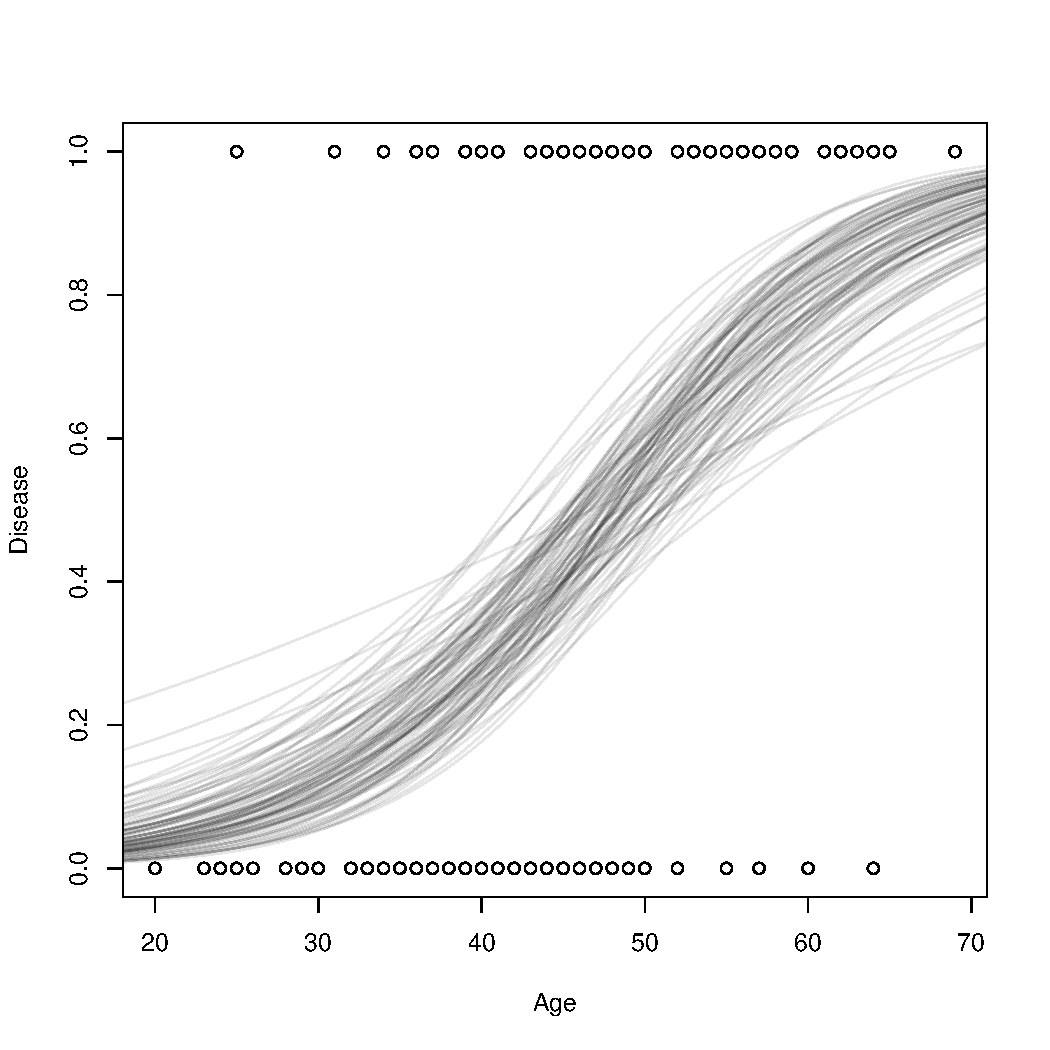
\includegraphics[width=0.6\textwidth]{images/logistic_curves.pdf}
\end{center}

\end{frame}


\begin{frame}
\frametitle{Informative Priors}

\begin{itemize}
\item We have mostly been using uniform or very wide normal priors,
and have been getting away with it.\pause
\item But they are actually a bit crazy, assigning probability to parameter
values we would never believe.\pause
\item We get away with it because the data is strong enough to rule out those
crazy values anyway.\pause
\item Thinking about the meaning of the parameter is often enough to let you
narrow down the priors a long way.
\end{itemize}

\end{frame}



\begin{frame}[fragile]
\frametitle{Informative Priors}

\begin{itemize}
\item $\beta_0$ is the value of the logit for a typical value of age,
since we centered \mintinline{r}{x}.
It probably shouldn't be too far outside the range $[-5, 5]$ (corresponding to
probabilities of about 0.007 to 0.993). \pause
\item People usually use normal distributions for informative priors, but I
disagree with that as they are very dogmatic --- the probability in the tails
is tiny.\pause
\item We can use the Student-$t$ distribution as an alternative:
\mintinline{r}{beta0 ~ dt(0, 1/3^2, 2)}.
\end{itemize}

\end{frame}


\begin{frame}[fragile]
\frametitle{Informative Priors}

\begin{itemize}
\item $\beta_1$ is the rate of change of logit per year of age. It
probably shouldn't be outside the range $[-1, 1]$
as this would lead to rapid change in disease probability over the course
of a single year of age --- implausible.\pause
\item $\beta_1$ is also almost certainly positive.\pause
\item Let's use \mintinline{r}{beta1 ~ dt(0.1, 1/1^2, 2)} so we expect
around 1 unit of logit change per decade of life, but with some uncertainty
that is still generous.
\end{itemize}

\end{frame}

\begin{frame}
\frametitle{Informative Priors}
\begin{itemize}
\item Despite having much narrower priors, the results of the parameter estimation
will be quite similar, because the data is `confirming' the priors.\pause
\item Informative priors are absolutely necessary for model comparison with
marginal likelihoods. The changes we just made would increase $Z$ by a factor
of about a million!\pause
\item As a sanity check (for mistakes in your thinking), you should check
that the posterior based on uniform priors isn't wildly inconsistent with
your informative priors.
\end{itemize}

\end{frame}


\begin{frame}
\frametitle{Poisson Regression}
Poisson regression is another `GLM'. It is just a regression model where
the sampling distribution is Poisson. We typically have the following:
\begin{align}
\lambda_i &= \exp\left(\beta_0 + \beta_1 x_i + \textnormal{extra terms}\right) \\
y_i \given \boldsymbol{\beta} &\sim \textnormal{Poisson}(\lambda_i)
\end{align}
Apart from priors, this is all we'll need for the JAGS code.

\end{frame}



\begin{frame}
\frametitle{Coal Data}
Let's revisit the coal data with this model (previously we had a change-point
model).

\begin{center}
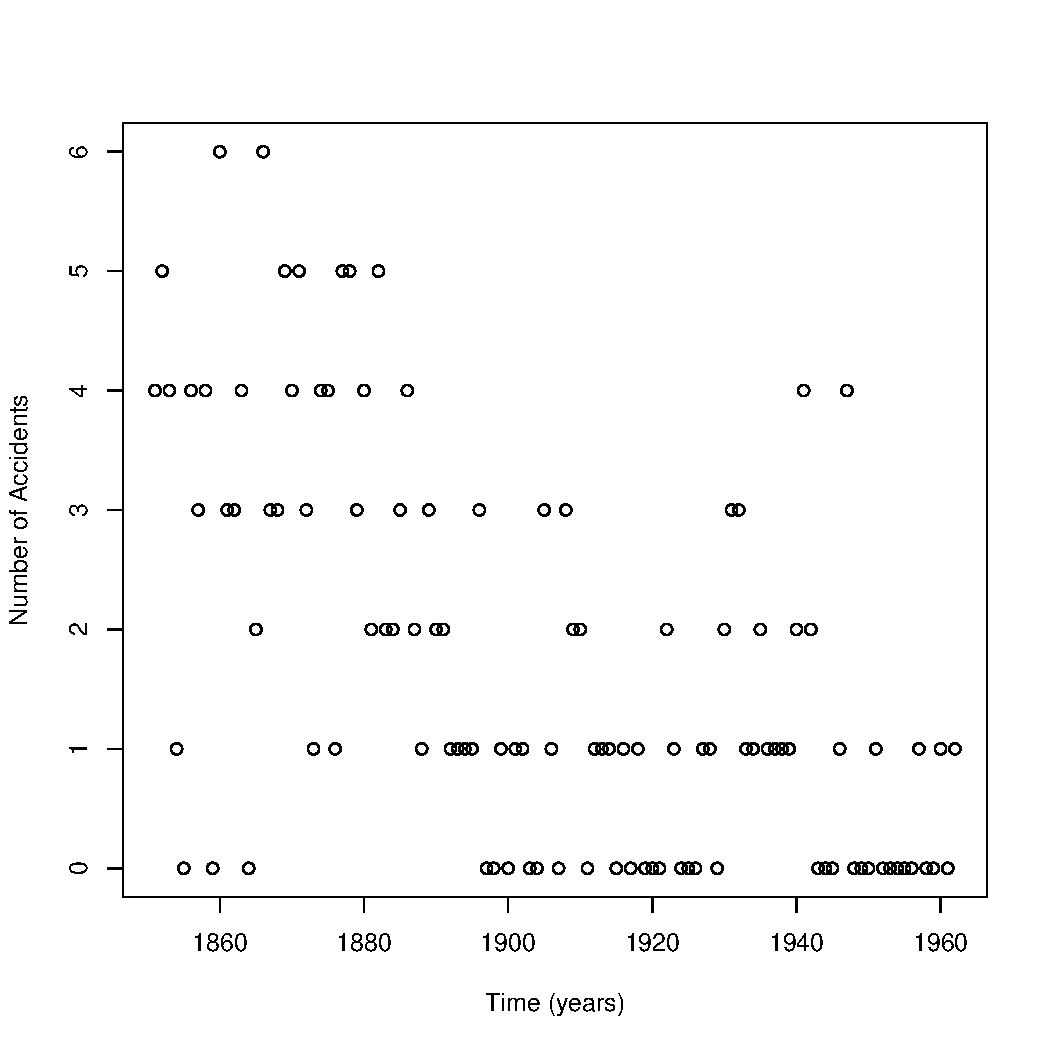
\includegraphics[width=0.4\textwidth]{images/coal.pdf}
\end{center}

\end{frame}


\begin{frame}[fragile]
\frametitle{Full JAGS Model with Priors}
Let's go back to being lazy about the priors, and remember that the
explanatory variable is called \mintinline{r}{t} in this dataset.
\footnotesize
\begin{minted}{r}
model
{
    beta0 ~ dnorm(0, 1/1000^2)
    beta1 ~ dnorm(0, 1/1000^2)

    for(i in 1:length(y))
    {
        lambda[i] <- exp(beta0 + beta1*(t[i] - mean(t)))
        y[i] ~ dpois(lambda[i])
    }
}
\end{minted}

\end{frame}


\begin{frame}[fragile]
\frametitle{Coal Results with GLM Assumptions}
We get the typical log-rate of accidents in the middle of the dataset
($\beta_0$) and the rate of change per year ($\beta_1$). We could tell from
the data that $\beta_1$ would be negative, and due to units it must be small.
\footnotesize
\begin{minted}{r}
> mean(results$beta0)
[1] 0.356763
> sd(results$beta0)
[1] 0.08454957
> mean(results$beta1)
[1] -0.01843049
> sd(results$beta1)
[1] 0.00247103
\end{minted}

\end{frame}


\begin{frame}[fragile]
\frametitle{Coal Results with GLM Assumptions}

\begin{center}
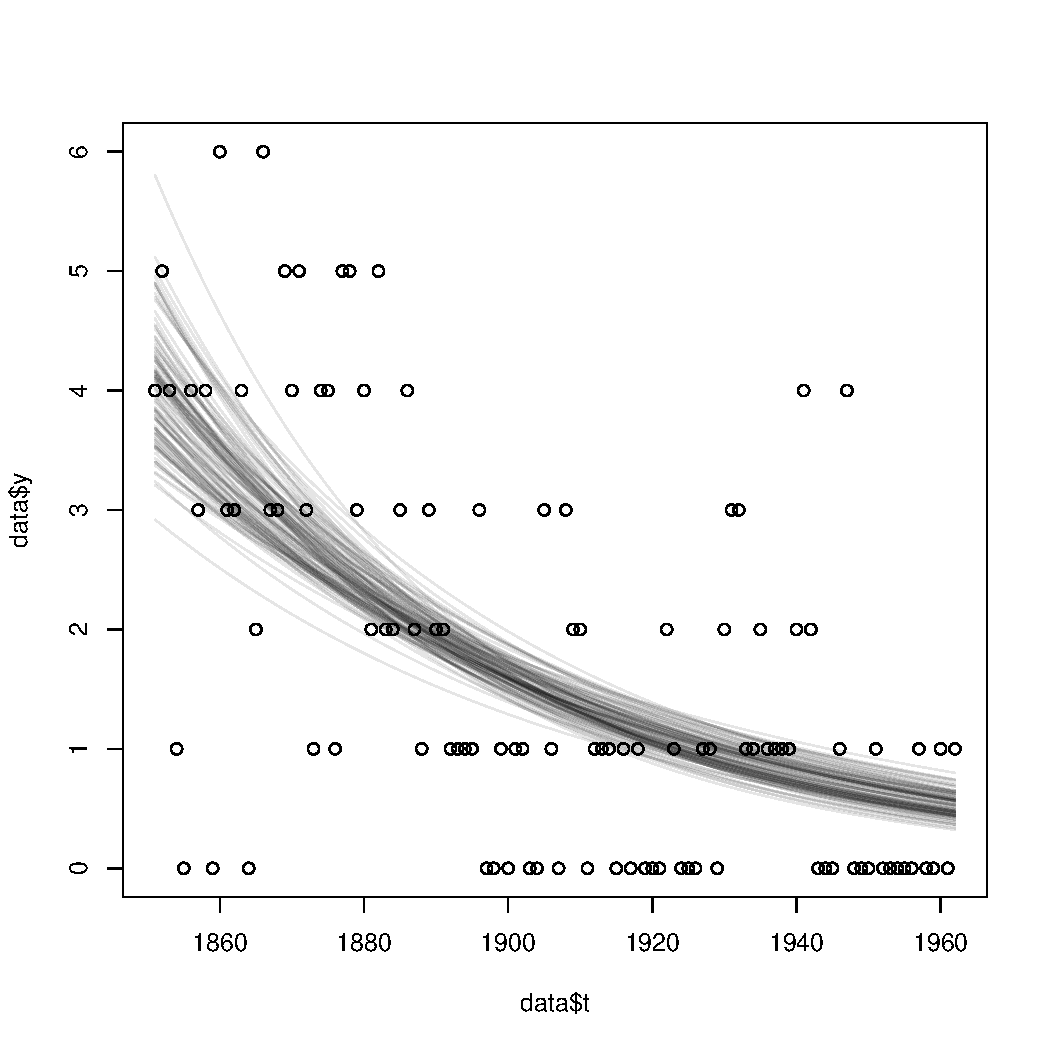
\includegraphics[width=0.6\textwidth]{images/coal_curves.pdf}
\end{center}
\end{frame}


\begin{frame}[fragile]
\frametitle{Coal Results: Code}

\begin{minted}{r}
t = seq(min(data$t), max(data$t), length=1000)
plot(data$t, data$y)
rows = sample(1:nrow(results), 100)
for(row in rows)
{
    lambda = exp(results$beta0[row] +
                 results$beta1[row]*(t - mean(data$t)))
    lines(t, lambda, col=rgb(0, 0, 0, 0.1))
}
\end{minted}
\end{frame}


\begin{frame}[fragile]
\frametitle{Coal Results}
Remember, we are not equipped to do {\bf model comparison} between the
change-point model and the GLM one. It is also not obvious how one might
do the alternative --- to put both ideas into a single parameter space.\\[0.5em]\pause

Other algorithms such as {\bf Nested Sampling} can do the model comparison
calculation.
\end{frame}


\begin{frame}
\frametitle{Negative Binomial Regression}
\begin{itemize}
\item The Poisson distribution is quite restrictive, as it asserts that if the
mean is $\lambda$ then the standard deviation must be $\sqrt{\lambda}$.
A two-parameter family might sometimes be better.\pause
\item For count data, the negative binomial is the traditional change to the
model to make it a bit more flexible than the Poisson, potentially to take
into account `overdispersion'.\pause
\item I will just show you how to use the negative binomial as a drop-in
replacement for the Poisson. It involves an extra parameter $r$, which,
if large, reproduces the Poisson approximately.
\end{itemize}

\end{frame}

\begin{frame}[fragile]
\frametitle{Negative Binomial Regression}
\footnotesize
\begin{minted}{r}
model
{
    beta0 ~ dnorm(0, 1/1000^2)
    beta1 ~ dnorm(0, 1/1000^2)
    log_r ~ dunif(0, 5) # Log-uniform prior for extra param
    r <- exp(log_r)

    for(i in 1:length(y))
    {
        lambda[i] <- exp(beta0 + beta1*(t[i] - mean(t)))
        p[i] <- r/(r + lambda[i])
        y[i] ~ dnegbin(p[i], r)
    }
}
\end{minted}

\end{frame}

\begin{frame}[fragile]
\frametitle{Negative Binomial Regression}
When we look at the posterior for \mintinline{r}{log_r} for the coal dataset
we see that high values are more plausible --- so the Poisson distribution
was actually fine (and would have been supported in a formal model comparison).

\end{frame}

\end{document}

